\documentclass[12pt, twoside]{article}
\usepackage[letterpaper, margin=1in, headsep=0.5in]{geometry}
\usepackage[english]{babel}
\usepackage[utf8]{inputenc}
\usepackage{amsmath}
\usepackage{amsfonts}
\usepackage{amssymb}
\usepackage{tikz}
\usetikzlibrary{quotes, angles}
\usepackage{graphicx}
%\usepackage{pgfplots}
%\pgfplotsset{width=10cm,compat=1.9}
%\usepgfplotslibrary{statistics}
%\usepackage{pgfplotstable}
%\usepackage{tkz-fct}
%\usepackage{venndiagram}
\usepackage{multicol}


\usepackage{fancyhdr}
\pagestyle{fancy}
\fancyhf{}
\fancyhead[RE]{\thepage}
\fancyhead[RO]{\thepage \\Name: \hspace{1.5in}.\\}
\fancyhead[LO]{BECA / Dr. Huson / Geometry 10th Grade\\* Unit 5: Transformation, dilation, and scale \\ 20 November 2019}

\renewcommand{\headrulewidth}{0pt}

\begin{document}
\subsubsection*{5.9 Do Now: Transformations and review}
  \begin{enumerate}

  \begin{multicols}{2}
    [\item A translation maps triangle $PQR$ onto triangle $STU$.] \vspace{0.5cm}
      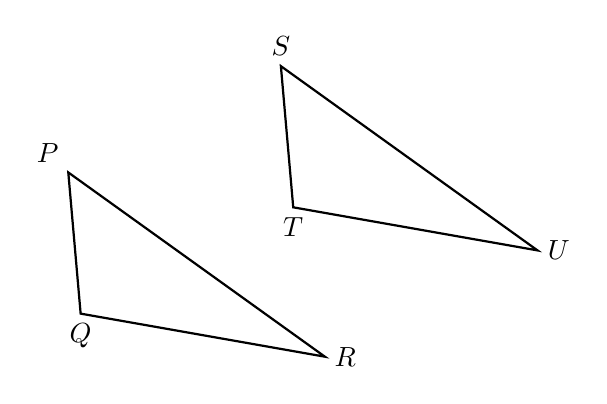
\begin{tikzpicture}[scale=0.9]
        \coordinate [label=above left:$P$](A) at (95:2);
        \coordinate [label=below:$Q$](B) at (0, 0);
        \coordinate [label=right:$R$](C) at (-10:3.5);
        \draw [thick] (A)--(B)--(C)--cycle;
  
        \draw [thick, xshift=3cm, yshift=1.5cm] (95:2) node[above]{$S$}--
        (0,0) node[below]{$T$}--
        (-10:3.5) node[right]{$U$}--cycle;
      \end{tikzpicture}\\
      Write each corresponding object.
      \begin{enumerate}
        \item $Q \rightarrow$ \rule{2cm}{0.15mm}
        \item $\angle QRP \cong$ \rule{2cm}{0.15mm}
        \item \rule{2cm}{0.15mm} $\cong \overline {ST}$
        \item Justify $\triangle PQR \cong \triangle STU$. Use the words ``rigid motion".
      \end{enumerate}
    \end{multicols}  \vspace{1cm}

  \begin{multicols}{2}
    [\item A dilation with $k=3$ centered at the origin maps $\triangle DEF$ onto $\triangle LMN$.] \vspace{0.5cm}
      The following is given:\\*[0.5cm]
      $DE=10$ \\
      $m\angle E = 40^\circ$ \\
      $m\angle F = 110^\circ$ \\
      $m\angle M = 2x + 10^\circ$ \\
      Fill in the blanks:
      \begin{enumerate}
        \item $D \rightarrow$ \rule{2cm}{0.15mm}
        \item $LM =$ \rule{2cm}{0.15mm}
        \item $m\angle M =$ \rule{2cm}{0.15mm}
        \item Solve for $x$
      \end{enumerate}
    \end{multicols}  \vspace{2cm}
  
   \item Triangle $ABC$ is dilated with a scale factor of $k$ centered at $A$, yielding $\triangle ADE$, as shown. Given $AB=8$, $BC=10$, $AC=12$, and $DE=15$. \\[0.25cm] Find $AD$, $CE$, and $k$ (the scale factor).
   \begin{flushright}
       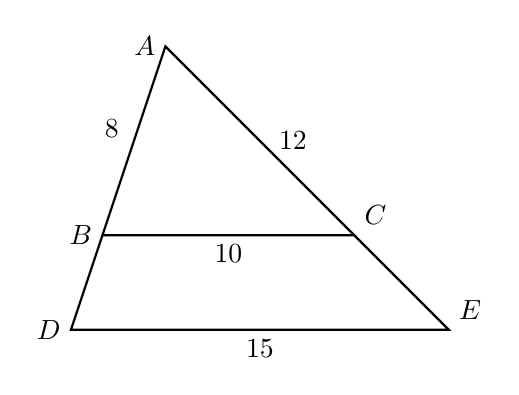
\begin{tikzpicture}[scale=0.4]
         \draw [thick]
         (0,0)node[left]{$B$}--
         (8,0)node[above right]{$C$}--
         (2,6)node[left]{$A$}--cycle;
         \draw [thick]
         (0,0)--
         (-1,-3)node[left]{$D$}--
         (11,-3)node[above right]{$E$}--(8,0);
         \node at (4,0)[below]{$10$};
         \node at (5.3, 3)[right]{$12$};
         \node at (0.3, 2.8)[above]{$8$};
         \node at (5,-3)[below]{$15$};
       \end{tikzpicture}
     \end{flushright}
  
\newpage

  \item What transformation maps $\triangle ABC$ onto $\triangle DEC$, shown below? Fully specify the transformation. \\[0.25cm]
    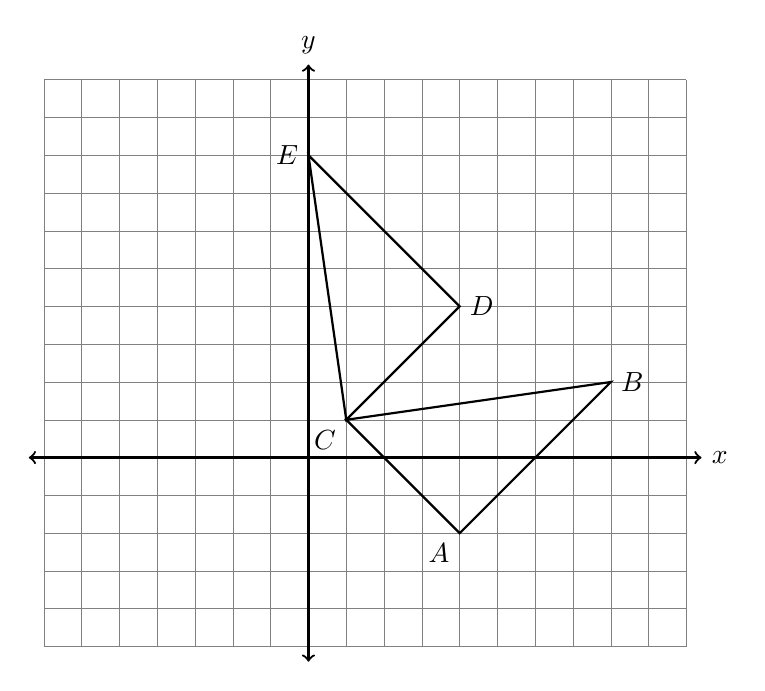
\begin{tikzpicture}[scale=.48]
      \draw [help lines] (-7,-5) grid (10,10);
      \draw [thick, <->] (-7.4,0) -- (10.4,0) node [right] {$x$};
      \draw [thick, <->] (0,-5.4)--(0,10.4) node [above] {$y$};  
      \draw [thick]
      (4,-2) node[below left] {$A$}--
      (8,2) node[right] {$B$}--
      (1,1) node[below left] {$C$}--cycle;  
      \draw [thick]
      (4,4) node[right] {$D$}--
      (0,8) node[left] {$E$}--
      (1,1) --cycle; 
    \end{tikzpicture}

  \item Given $\triangle JKL \sim \triangle MNO$. $m\angle K = 40^\circ$ and $m\angle M = 100^\circ$.\\
  Find the measure of $\angle N$. \vspace{3cm}

  \item Given isosceles $\triangle ABC$ with $\overline{AC} \cong \overline{AB}$, $m\angle A = x$, $m\angle B = 55$, and $m\angle C=y$. Find $x$ and $y$. \hfill (\emph{the diagram is not to scale})
  \begin{flushright}
  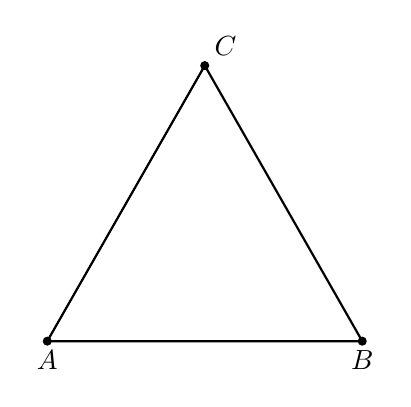
\begin{tikzpicture}[scale=1]
    \draw [thick](0,0)--(4,0)--(2,3.5)--(0,0);
    \draw [fill] (0,0) circle [radius=0.05] node[below]{$A$};
    \draw [fill] (4,0) circle [radius=0.05] node[below]{$B$};
    \draw [fill] (2,3.5) circle [radius=0.05] node[above right]{$C$};
  \end{tikzpicture}
  \end{flushright}

\newpage 

  \item Given isosceles $\triangle RSU$ with $\overline{UR} \cong \overline{RS}$. If $m\angle UST=140$ find $m\angle U$.
  \begin{flushright}
  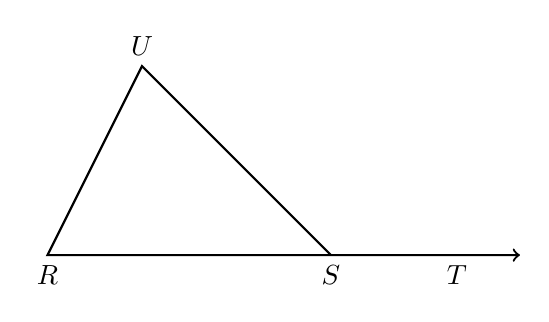
\begin{tikzpicture}[scale=0.8]
    %\draw [->, thick] (0,0)--(5,5);
    \draw [<-, thick] (8,0)--
      (7,0) node[below]{$T$}--
      (0.5,0) node[below]{$R$}--
      (2,3) node[above]{$U$}--
      (5,0) node[below]{$S$};
  \end{tikzpicture}
  \end{flushright} \vspace{1cm}

  \item Translate $\triangle ABC$ by $(x,y) \rightarrow (x+3, y+4)$. Make a table of the coordinates and plot and label the image on the axes.
  \begin{flushright}
      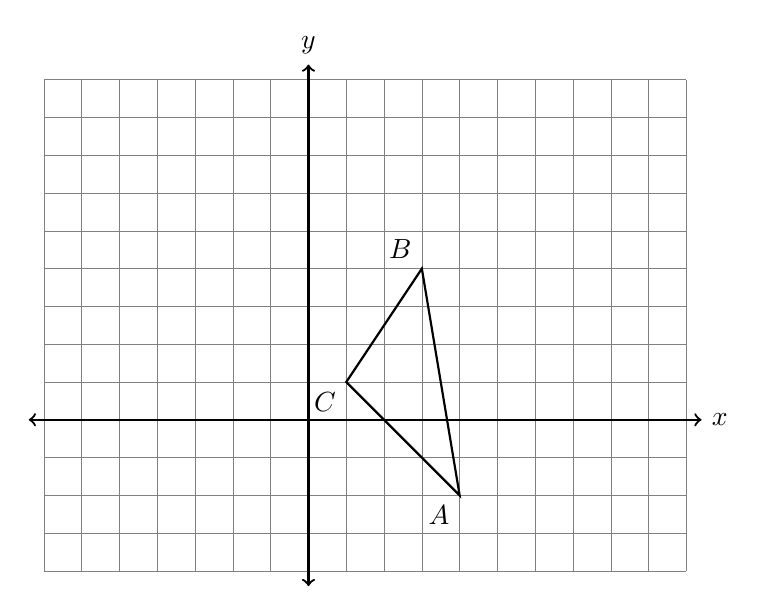
\begin{tikzpicture}[scale=.48]
      \draw [help lines] (-7,-4) grid (10,9);
      \draw [thick, <->] (-7.4,0) -- (10.4,0) node [right] {$x$};
      \draw [thick, <->] (0,-4.4)--(0,9.4) node [above] {$y$};  
      \draw [thick]
        (4,-2) node[below left] {$A$}--
        (3,4) node[above left] {$B$}--
        (1,1) node[below left] {$C$}--cycle;  
    \end{tikzpicture}
  \end{flushright}

  \item Two parallel lines intersect a second set of parallel lines. Given $m\angle 1 = x$ and $m\angle 2 = x+50$, find the measure of $\angle 4$. 
    \begin{flushright}
      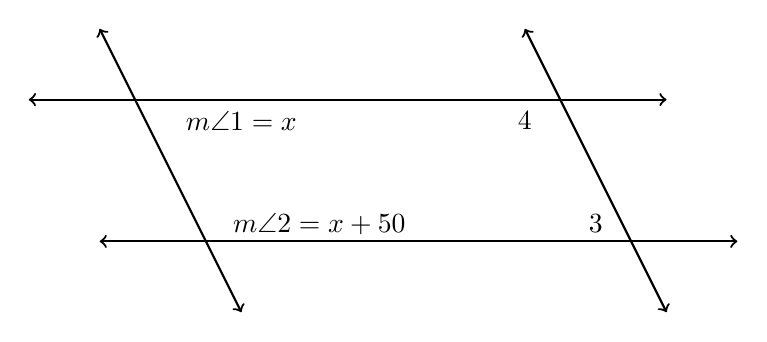
\begin{tikzpicture}[scale=0.9]
        \draw [<->, thick] (3,0)--(12,0);
        \draw [<->, thick] (2,2)--(11,2);
        \draw [<->, thick] (5,-1)--(3,3);
        \draw [<->, thick] (11,-1)--(9,3);
        \node at (5, 1.7){$m\angle 1 = x$};
        \node at (6.1, 0.25){$m\angle 2 = x+50$};
        \node at (10, 0.25){$3$};
        \node at (9, 1.7){$4$};
      \end{tikzpicture}
    \end{flushright}

\newpage
  \item Using a compass and straightedge, construct the perpendicular bisector of $\overline{BB'}$  \\[0.25cm]
  What transformation has been applied to map $\triangle ABC$ on to $\triangle A'B'C'$? \vspace{2cm}
      \begin{center}
      \begin{tikzpicture}%[scale=.48]
        %\draw [thick, <->] (-7.4,0) -- (10.4,0) node [right] {$x$};
        %\draw [thick, <->] (0,-6.4)--(0,10.4) node [above] {$y$};
        \draw [thick]
          (5,-1) node[below left] {$A$}--
          (8,2) node[right] {$B$}--
          (1,0) node[below left] {$C$}--cycle;
        \draw [thick]
          (-1,5) node[right] {$A'$}--
          (2,8) node[above] {$B'$}--
          (0,1) node[below left] {$C'$}--cycle;
      \end{tikzpicture}
    \end{center}

    \item Given parallel lines $\overleftrightarrow{AB} \parallel \overleftrightarrow{CDE}$ with $\overline{AC} \cong \overline{AD}$. If $m\angle BAD=70$ find $m\angle ACD$.
    \begin{flushright}
    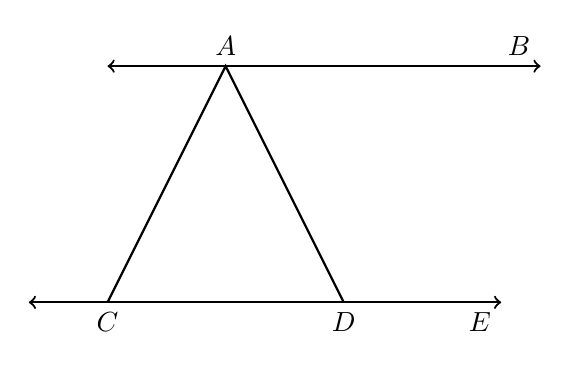
\begin{tikzpicture}
      \draw [<->, thick] (1,3)--(6.5,3) node[above left]{$B$};
      \draw [<->, thick] (0,0)--
        (5,0)--
        (6,0) node[below left]{$E$};
      \draw [-, thick] (1,0) node[below]{$C$}--
        (2.5,3) node[above]{$A$}--
        (4,0) node[below]{$D$};
    \end{tikzpicture}
    \end{flushright} \vspace{1.5cm}

\end{enumerate}
\end{document}
